%----------------------------------------------------------------------------------------
%	PRESENTATION SLIDES Section 2
%----------------------------------------------------------------------------------------
\section{Logistic Regression} 

\begin{frame}
\huge{\centerline{Section 2: Logistic Regression Model}}
\end{frame}
%------------------------------------------------
\subsection{Iris Flower}
\begin{frame}
\frametitle{Fisher's Iris}
The data set consists of 50 samples from each of three 
species of iris flowers.  Four features were measured from each
sample, they are the length and the width of sepal and petal. This data set is often used
to demonstrate classification techniques and discriminant analysis.

\begin{figure}
\centering
\begin{subfigure}{.3\textwidth}
  \centering
  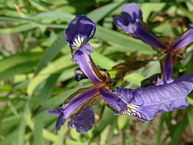
\includegraphics[scale=.45]{graphics/setosa}
  \caption{setosa}
  \label{fig:sub1}
\end{subfigure}%
\begin{subfigure}{.3\textwidth}
  \centering
  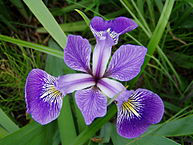
\includegraphics[scale=.45]{graphics/versicolor}
  \caption{versicolor}
  \label{fig:sub2}
\end{subfigure}
% 
\begin{subfigure}{.3\textwidth}
  \centering
  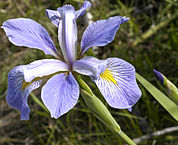
\includegraphics[scale=.45]{graphics/virginica}
  \caption{virginica}
  \label{fig:sub2}
\end{subfigure}
\label{fig:test}
\end{figure}


\end{frame}

%------------------------------------------------
\begin{frame}
\frametitle{Fisher's Iris}
Four features were measured from each
sample, they are the length and the width of sepal and petal.
\begin{figure}[htbp]
\centering
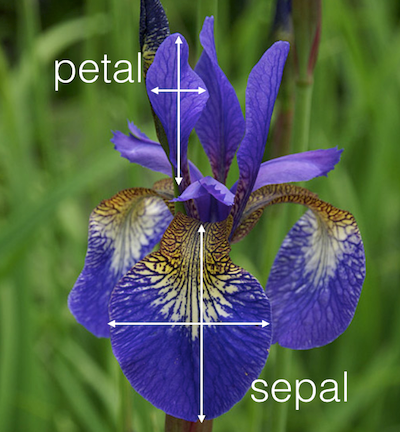
\includegraphics[scale=.35]{graphics/iris_feature} \caption{Features}
\label{fig:Features}
\end{figure}
\end{frame}
%------------------------------------------------
\begin{frame}
\frametitle{Sample Data}

\begin{table}
\begin{tabular}{lllll}
\hline
\textbf{Sepal Length} & \textbf{ Sepal Width } & \textbf{Petal Length} & \textbf{Petal Width} & \textbf{Species}\\
\hline
5.8 & 4.0 & 1.2 & 0.2 & setosa\\
6.4 & 2.8 & 5.6 & 2.1 & virginica\\
6.7 & 3.1 & 5.6 & 2.4 & virginica \\
\hline
\end{tabular}
\caption{Fisher's Iris Dataset Sample}
\end{table}

\begin{figure}[htbp]
\centering
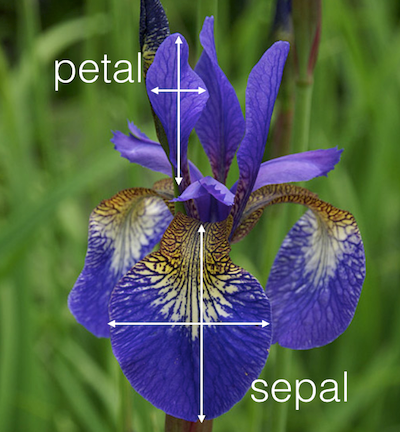
\includegraphics[scale=.23]{graphics/iris_feature} \caption{Features}
\end{figure}


\end{frame}
%------------------------------------------------
\begin{frame}
\frametitle{Visualization of Iris Dataset}
\begin{figure}[t]
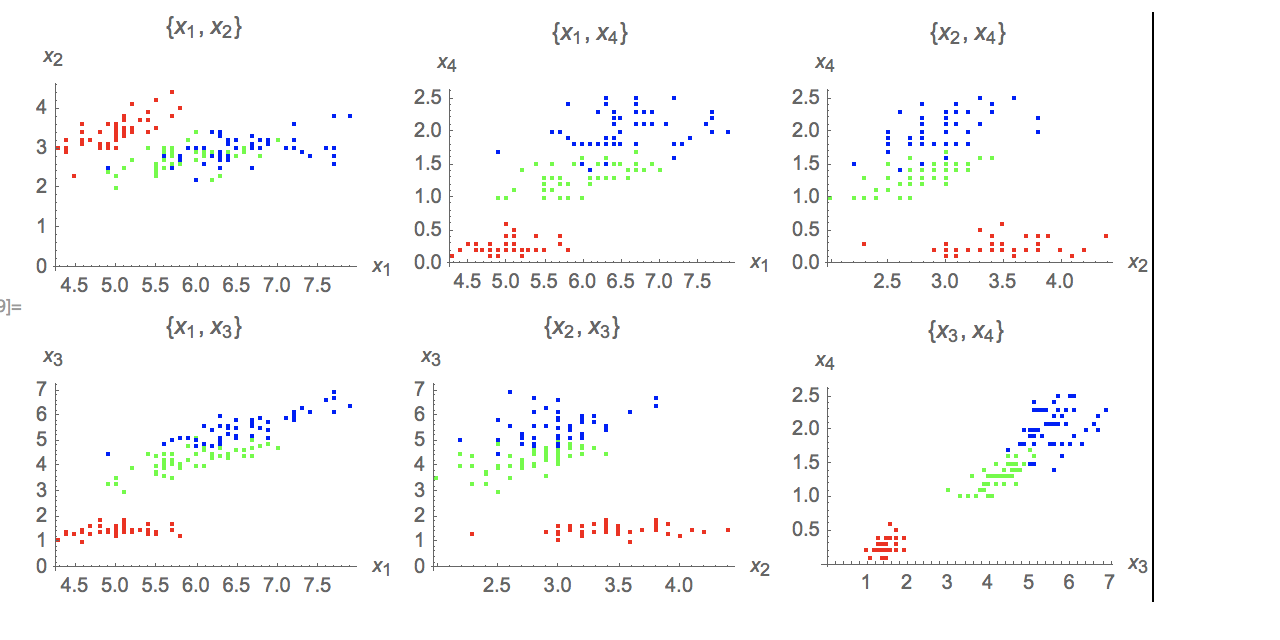
\includegraphics[scale=0.5]{graphics/feature_vis}
\centering
\end{figure}
\end{frame}
%------------------------------------------------
\begin{frame}
\frametitle{}
\[\text{Let's start from binary classification y $\in $ $\{$0, 1$\}$}\]

\[\text{y $\in $ $\{$0, 1$\}$   where 0 $\to $ versicolor 1$\to $ virginica}\]
\[	
	\mathbf{x} = (x_ 1, x_ 2) \
		where \ x_1 = \text{sepal width}, x_2 = \text{petal width}\]
		
% ----------
\begin{figure}
\begin{subfigure}{.4\textwidth}
  \centering
  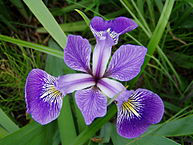
\includegraphics[scale=.5]{graphics/versicolor}
  \caption{versicolor}
  \label{fig:sub1}
\end{subfigure}
% 
\begin{subfigure}{.4\textwidth}
  \centering
  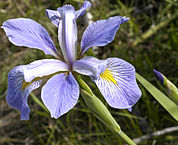
\includegraphics[scale=.5]{graphics/virginica}
  \caption{virginica}
  \label{fig:sub2}
\end{subfigure}
\label{fig:test}
\end{figure}
% ----------
\end{frame}
%------------------------------------------------
\subsection{Sigmoid Function}
\begin{frame}
\frametitle{Sigmoid Function}
\[\sigma(x)=\frac{1}{1+e^{-x}}\]
\begin{figure}[t]
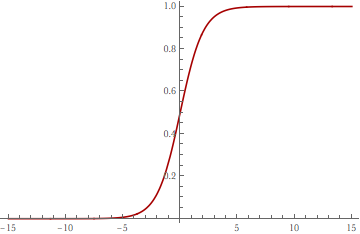
\includegraphics[width=5cm]{graphics/1d-sigmoid}
\centering
\end{figure}
\end{frame}
%------------------------------------------------
\begin{frame}
\begin{multicols}{2} % 2 columns
\begin{figure}[t]
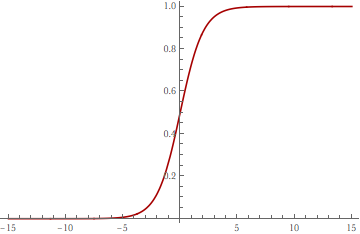
\includegraphics[width=5cm]{graphics/1d-sigmoid}
\centering
\end{figure}
\columnbreak  % seperate
In this example, you can think 
\[ \bm{\theta} = (\theta_{0}, \theta_{1}) \ and \ \mathbf{x} = (1, x)\]
therefore, 
\[p(\mathbf{x} ;  \bm{\theta}) =  \frac{1}{1+e^{- ( \theta_{0} +  \theta_{1} \cdot  x )}} \]
\\
\end{multicols}
\begin{multicols}{2}
\[p(x;  \bm{\theta}) \geq \frac{1}{2}  \Rightarrow class 1\]
\[p(x;  \bm{\theta})<\frac{1}{2}  \Rightarrow class 0\]
\columnbreak 
\[p(\mathbf{x};  \bm{\theta})=P(y=1|\mathbf{x}) = \frac{1}{1+e^{-\bm{\theta} ^ {\intercal} \mathbf{x}}}\]
\[1-p(\mathbf{x};  \bm{\theta})=P(y=0|\mathbf{x}) = \frac{e^{-\bm{\theta} ^ {\intercal} \mathbf{x}}} {1+e^{-\bm{\theta}^\intercal \mathbf{x}}} \]
\end{multicols}
\end{frame}
%------------------------------------------------ 
\begin{frame}
\begin{centering}
\begin{equation}
\begin{aligned}
class 1 &\Leftrightarrow p(\mathbf{x};  \bm{\theta}) = \frac{1}{1+e^{-\bm{\theta} ^ {\intercal} \mathbf{x}}} > \frac{1}{2} \\
&\Leftrightarrow e^ {-\bm{\theta} ^ {\intercal} \mathbf{x}} > 1\\
&\Leftrightarrow \bm{\theta} ^ {\intercal} \mathbf{x} > 0\\
\end{aligned}
\end{equation}
\\
\begin{equation}
\begin{aligned}
class 0 &\Leftrightarrow p(\mathbf{x};  \bm{\theta}) = \frac{1}{1+e^{-\bm{\theta} ^ {\intercal} \mathbf{x}}} < \frac{1}{2} \\
&\Leftrightarrow e^ {-\bm{\theta} ^ {\intercal} \mathbf{x}} < 1\\
&\Leftrightarrow \bm{\theta} ^ {\intercal} \mathbf{x} < 0\\
\end{aligned}
\end{equation}
\end{centering}
%\[p(\mathbf{x}) = \frac{1}{1+e^{-\bm{\theta \intercal} \mathbf{x}}} \geq \frac{1}{2} \Leftrightarrow \bm{\theta \intercal} \mathbf{x} > 0 \Rightarrow class 1\]
%\[p(\mathbf{x}) = \frac{1}{1+e^{-\bm{\theta \intercal} \mathbf{x}}} <\frac{1}{2}  \Leftrightarrow \bm{\theta \intercal} \mathbf{x} < 0 \Rightarrow class 0\]
\\
\begin{block}{Conclusion}
\begin{itemize}
\item Logistic regression gives us a \textbf{linear classifier}. \\
\item $\bm{\theta}  ^\intercal \mathbf{x} = 0$ is \textbf{decision boundary}. 
\end{itemize}
\end{block}
\end{frame}
%------------------------------------------------
\begin{frame}
3D Visualization \\
See a Mathematica Dynamic Visualization
\end{frame}
%------------------------------------------------
\subsection{Likelihood Function for Logistic Regression}
\begin{frame}
\frametitle{Maximum Likelihood}

We can assume that
\[P(y = 1 | \mathbf{x}) = p(\mathbf{x}; \bm{\theta})\]
\[P(y = 0 | \mathbf{x}) = 1- p(\mathbf{x}; \bm{\theta})\]

The likelihood function $\mathcal{L}$, which quantifies how likely output is given input, is defined as follows:
% likelihood
\begin{equation}
\begin{aligned}
\mathcal{L}(\bm{\theta}) &= \prod_{i=1}^n P(Y = y_{i}  | X = \mathbf{x}_{i}; \bm{\theta}) = \prod_{y_{i} = 0 } (1-p(\mathbf{x}_{i}; \bm{\theta})) \prod_{y_{i} = 1 } (p(\mathbf{x}_{i}; \bm{\theta})) \\
&= \prod_{i=1}^{n} p(\mathbf{x}_{i}; \bm{\theta})^{y_{i}} (1-p(\mathbf{x}_{i}; \bm{\theta}))^{(1-{y_{i}})}
\end{aligned}
\end{equation}
\end{frame}

%------------------------------------------------
\begin{frame}
\frametitle{Maximum Likelihood}

% likelihood
\begin{equation}
\begin{aligned}
\mathcal{L}(\bm{\theta}) &= \prod_{i=1}^n P(Y = y_{i}  | X = \mathbf{x}_{i}, \bm{\theta}) = \prod_{y_{i} = 0 } (1-p(\mathbf{x}_{i}; \bm{\theta})) \prod_{y_{i} = 1 } (p(\mathbf{x}_{i}; \bm{\theta})) \\
&= \prod_{i=1}^{n} p(\mathbf{x}_{i}; \bm{\theta})^{y_{i} }(1-p(\mathbf{x}_{i}; \bm{\theta}))^{(1-{y_{i}})}
\end{aligned}
\end{equation}

\begin{equation}
\begin{aligned}
\ell (\bm{\theta}) &=  \log (\mathcal{L}(\bm{\theta}) ) = \sum_{i=1}^{n} y_{i} \log(p(\mathbf{x}_{i}; \bm{\theta}) + (1-y_{i}) \log(1-p(\mathbf{x}_{i}; \bm{\theta})) \\
&= \sum_{y_{i} = 0 } \log (1-p(\mathbf{x}_{i}; \bm{\theta})) + \sum_{y_{i} = 1} \log (p(\mathbf{x}_{i}; \bm{\theta})) \\
\end{aligned}
\end{equation}

Since $f(x) = log(x)$ is a monotonically increasing function, maximizing $\mathcal{L}(\bm{\theta})$ is equivalent as maximizing $\ell(\bm{\theta})$
\end{frame}
%------------------------------------------------
\begin{frame}
\frametitle{Maximum Likelihood Estimation}
Set derivatives equal to zero, then solve, we will find the maximum likelihood.
Let $p(\mathbf{x}) = \sigma(\bm{\theta}^{\intercal} \mathbf{x}) = \frac{1}{1+ e^{-\bm{\theta}^{\intercal} \mathbf{x}}}$

\begin{equation}
\begin{aligned}
\ell'(\bm{\theta}) 
&= \frac{\partial \ell}{\partial \bm{\theta}} =\left(y \frac{1}{\sigma(\bm{\theta}^{\intercal} \mathbf{x})} - (1-y) \frac{1}{1-\sigma(\bm{\theta}^{\intercal} \mathbf{x})}\right) 
\frac{\partial }{\partial \bm{\theta}_{j}} \sigma(\bm{\theta}^{\intercal} \mathbf{x}) \\
&= \left(y \frac{1}{\sigma(\bm{\theta}^{\intercal} \mathbf{x})} - (1-y) \frac{1}{1-\sigma(\bm{\theta}^{\intercal} \mathbf{x})}\right) 
\sigma(\bm{\theta}^{\intercal} \mathbf{x})(1-\sigma(\bm{\theta}^{\intercal} \mathbf{x})) 
\frac{\partial }{\partial \bm{\theta}_{j}} \bm{\theta}^{\intercal} \mathbf{x} \\
&= \left(y(1-\sigma(\bm{\theta}^{\intercal} \mathbf{x}) - (1-y) \sigma(\bm{\theta}^{\intercal} \mathbf{x}) \right) \mathbf{x}_{j} \\
&= (y - p(\mathbf{x}))\mathbf{x}_{j}
\end{aligned}
\end{equation}

Solve for $\bm{\theta}$ by setting $\ell'(\bm{\theta}) =0$ \\
Let's go back to our iris flower and take a look of a concrete example!
\end{frame}
%------------------------------------------------
\subsection{Logistic Regression with More Than Two Classes}
\begin{frame}
\frametitle{Logistic Regression with More Than Two Classes}
If $Y$ can take on $k$ values, i.e. we have $k$ classes, we can still use logistic regression. The predicted conditional probabilities will be 
\begin{equation}
P(Y = c | X = \mathbf{x}) = \frac{\exp ({{\bm{\theta}}^{c}}^ {\intercal} \mathbf{x})} { \sum_{j}^{k} \exp({{\bm{\theta}}^{j}}^ {\intercal}\mathbf{x}) }
\end{equation}
This is commonly known as Softmax function.
\end{frame}
%------------------------------------------------
\subsection{More Topics About Logistic Regression}
\begin{frame}
\large{\centerline{More topics about logistic regression..}}
\end{frame}

%----------------------------------------
% The Math of March Madness
%--------------------------------------
% Frame 1
\begin{frame}
\frametitle{The Math of March Madness}
\begin{figure}

\includegraphics[width=0.8\linewidth]{Math_of_march_madness.png}
\end{figure}
\end{frame}

% Frame 2
\begin{frame}
\frametitle{The Math of March Madness}
\begin{itemize}
\item \say{\textit{Professors Lopez and Matthews didn't use any of the au courant methods in data science circles, either: no deep learning, no hierarchical clustering, no compressed sensing; just a good old model called \textbf{logistic regression}, which turns a number (like a point spread) into an estimated probability that team A will beat team B.}}
\end{itemize}
\end{frame}

% Frame 3
\begin{frame}
\frametitle{The Math of March Madness}
\begin{itemize}
\item Just 2 data sources used - the Las Vegas point spreads for the N.C.A.A. match-ups and a set of offensive and defensive efficiency ratings. 
\item Shows that if the data is simple, then logistic regression can be an efficient algorithm - compared to more complex methods which may easily overfit.
\end{itemize}
\end{frame}

% --------------------------
% Relation with cross-entropy
% --------------------------
% Frame 1
\begin{frame}
\frametitle{Relation with Cross-entropy Error Measure}
\begin{itemize}
\item For two probability distributions $\{p,1-p\}$ and $\{q,1-q\}$ with binary outcomes, the \textit{cross-entropy} (from information theory) 
\begin{equation}
\begin{split}
&= p \log \frac{1}{q} + (1-p) \log \frac{1}{1-q}\\
&= -p \log q - (1-p) \log (1-q)
\end{split}
\end{equation}
\item Assuming that $p$ is the \say{true} distribution and $q$ is the approximate distribution for $p$, minimizing the cross-entropy is equivalent to minimizing the distance (KL-divergence) between the 2 distributions,  i.e. make the approximate distribution as close to the "true" distribution as possible.
\end{itemize}
\end{frame}

% Frame 2
\begin{frame}
\frametitle{Relation with Cross-entropy Error Measure}
\begin{itemize}
\item For the $i^{th}$ training data,
\begin{equation}
\begin{split}
p_i &= y_i \\
q_i &= \sigma (\theta^T \mathbf{x}_i)
\end{split}
\end{equation}
\item The negative log likelihood for the $i^{th}$ training data point may be expressed as
\begin{equation}
-\log P(Y=y_i|X=\mathbf{x_i}) = -y_i \log \sigma (\theta^T \mathbf{x}_i) - (1-y_i) \log (1-\sigma (\theta^T \mathbf{x}_i))
\end{equation}
\item Same as cross-entropy measure.
\end{itemize}
\end{frame}

% Frame 3
\begin{frame}
\frametitle{Relation with Cross-entropy Error Measure}
\begin{itemize}
\item Total cross-entropy error measure over all data points is equal to the negative log likelihood for observation $Y$ given training data set $\mathbf{x}$ and $\theta$, i.e. the cost function for the logistic regression model.
\item Minimizing the cost function w.r.t. $\theta$ may thus be also interpreted as minimizing the distance between the \say{true} distribution (i.e. observation) and the sigmoid approximation.

\end{itemize}
\end{frame}


%------------------------------------------------
% Regularization
%------------------------------------------------
% Frame 1
\subsection{Regularization}
\begin{frame}
\frametitle{Regularization}
\begin{itemize}
\item \textbf{Bayesian view:} If the parameters are assumed to have a prior distribution, then we need to perform \textit{maximum a posteriori} (MAP) estimation.
\item Recall, Bayes' theorem:
\begin{equation}
posterior \propto likelihood \times prior
\end{equation}
\item If the parameters are assumed to have a prior distribution, then we need to perform \textit{maximum a posteriori} (MAP) estimation.
\end{itemize}
\end{frame}
%--------------------------------------------------
\begin{frame}
\frametitle{Regularization}
\begin{itemize}
\item Let $P(\mathbf{\theta}) = \text{exp}(-\frac{||\mathbf{\theta}||^2}{2 \sigma^2})$. Then
\begin{equation}
\begin{split}
\mathbf{\theta}^* &= \text{argmax} (\prod_{i=1}^n P(y_i|\mathbf{x_i, \theta}) P(\mathbf{\theta}))\\
&= \text{argmin} (-\log (\prod_{i=1}^n P(y_i|\mathbf{x_i, \theta}) P(\mathbf{\theta})))\\
&= \text{argmin} (-\log (\prod_{i=1}^n P(y_i|\mathbf{x_i, \theta}) - \log P(\theta))\\
&= \text{argmin} (-\log (\prod_{i=1}^n P(y_i|\mathbf{x_i, \theta}) + \frac{||\mathbf{\theta}||^2}{2 \sigma^2})
\end{split}
\end{equation}
\end{itemize}
\end{frame}
%------------------------------------------------
\begin{frame}
\frametitle{Regularization}
\begin{itemize}
\item Replacing $\lambda = \frac{1}{2 \sigma^2}$, the MAP estimator minimizes the negative log-likelihood added with an L2 regularization term.
\item Adding a regularization term prevents overfitting by increasing training error but reducing generalization error. $\lambda$ controls the extent of regularization.
\item Reduces model complexity by enforcing constraints on parameters.
\item Varying the prior function leads to different types of regularization, e.g. a Laplacian prior produces L1 regularization.
\end{itemize}
\end{frame}
%------------------------------------------------
\begin{frame}
\frametitle{Regularization}
\begin{itemize}
\item Illustration:
\end{itemize}
\begin{figure}
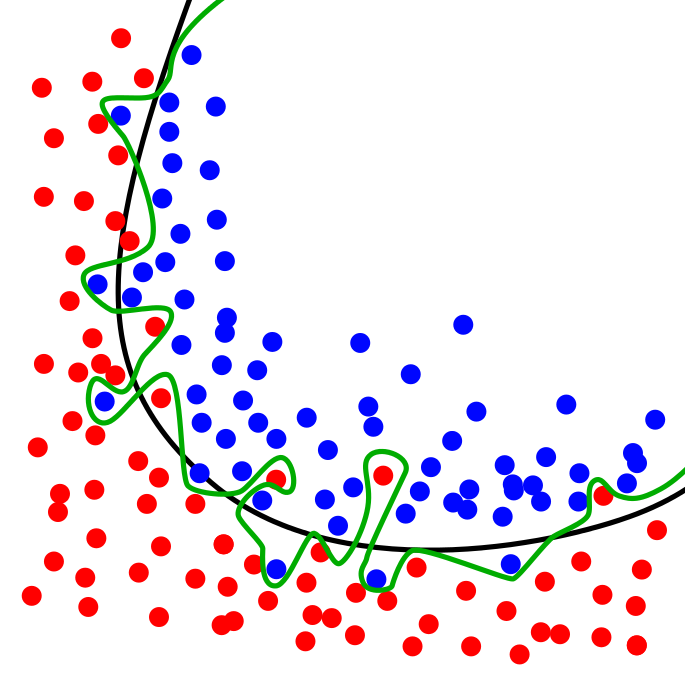
\includegraphics[width=0.5\linewidth]{overfitting.png}
\end{figure}
\end{frame}
%------------------------------------------------
\begin{frame}
\frametitle{Regularization}
\begin{itemize}
\item 
\begin{equation}
\text{min} \hspace{0.1in} J(\theta) + \lambda_C \theta^T \theta
\end{equation}
where $\lambda_C$ is the Lagrangian multiplier.
\item Lagrangian form of constrained optimization problem:
\begin{align}
\text{min} &\hspace{0.1in} J(\theta)\\
\text{s.t.} &\hspace{0.1in} \theta^T \theta \leq C
\end{align}
\end{itemize}
\end{frame}
%-------------------------------------------------
% LR and Neural networks
\subsection{To Neural networks}
\begin{frame}
\frametitle{Logistic Regression and Neural Networks}
\begin{itemize}
\item Logistic regression may be thought of as a single-layer neural network with a sigmoid activation function.
\begin{figure}
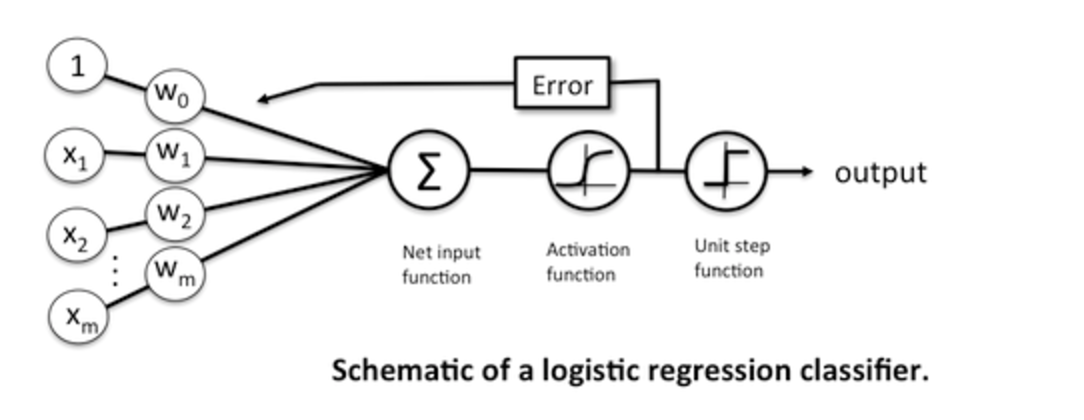
\includegraphics[width=0.8\linewidth]{LR_NN.png}
\end{figure}
\end{itemize}
\end{frame}
%------------------------------------------------
\begin{frame}
\frametitle{Logistic Regression and Neural Networks}
\begin{itemize}
\item Neural networks may be visualized as a combination of linear classifiers for complex boundaries.
\item Example: XOR function
\begin{figure}
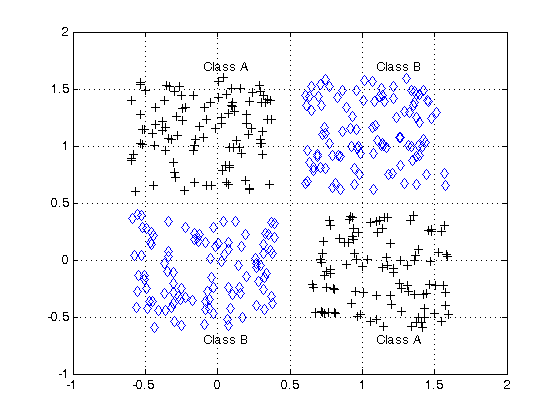
\includegraphics[width=0.6\linewidth]{xor_image.png}
\end{figure}
\end{itemize}
\end{frame}
%------------------------------------------------
\begin{frame}
\frametitle{Logistic Regression and Neural Networks}
\begin{itemize}
\item Sigmoid activation function commonly used previously in hidden layers of neural networks along with \textit{softmax} (multinomial logistic regression) at the final fully connected output layer. 
\item Nowadays, ReLU (\textbf{Re}ctified \textbf{L}inear \textbf{U}nit) activation function is most popular, but softmax is still commonly used at the final layer.
\begin{figure}
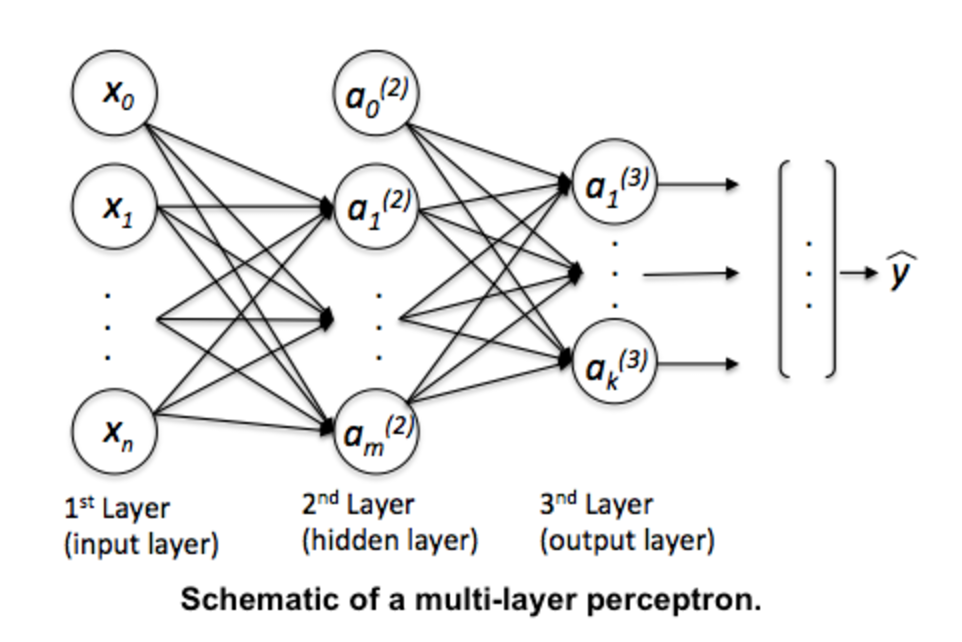
\includegraphics[width=0.5\linewidth]{MLP.png}
\end{figure}
\end{itemize}
\end{frame}
%------------------------------------------------
\begin{frame}
\frametitle{Logistic Regression and Neural Networks}
\begin{itemize}
\item Logistic regression cost function is convex, but cost function of neural networks is non-convex due to combination of multiple logistic regression layers.
\begin{figure}
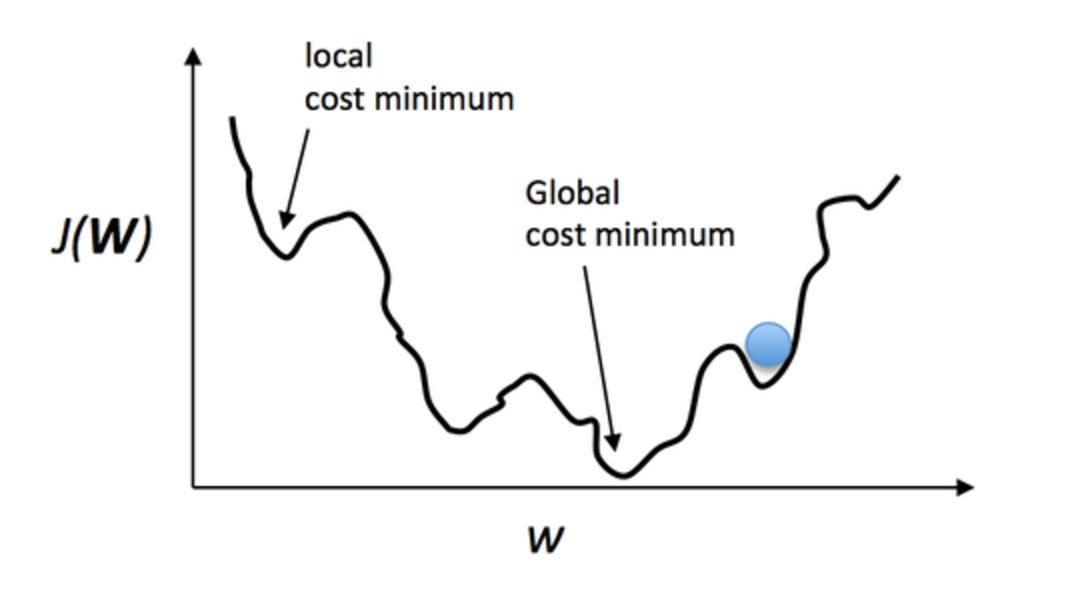
\includegraphics[width=0.7\linewidth]{NN_cost.png}
\end{figure}
\end{itemize}
\end{frame}